\documentclass[mathserif]{beamer}
\newcommand{\be}{\begin{equation}}
\newcommand{\ee}{\end{equation}}
\newcommand{\bce}{\begin{center}}
\newcommand{\ece}{\end{center}}
\newcommand{\dpa}[2]{\frac{\partial #1}{\partial #2}}
\newcommand{\ndp}[3]{\frac{\partial^#3 #1}{\partial #2 ^#3}}
\newcommand{\cdpa}[3]{\frac{\partial^2 #1}{\partial #2 \partial #3}}
\usepackage[utf8]{inputenc}
\usepackage{ragged2e}
\usepackage{etoolbox}
\usepackage{animate}
\usepackage{booktabs}
\usepackage{eulervm}
\apptocmd{\frame}{}{\justifying}{}
\usepackage[activeacute,spanish]{babel}
\setbeamertemplate{navigation symbols}{}
\setbeamertemplate{caption}[numbered]
\usetheme{default}
\setbeamertemplate{footline}[frame number]
\definecolor{cobalt}{rgb}{0.0, 0.28, 0.67}
\usecolortheme[named=cobalt]{structure}
\setbeamercolor{alerted text}{fg=blue}
\title{Simulación Multiescala de Viento Sobre Terreno Complejo Mediante el Método Embedido WRF-LES y Asimilación Variacional de Datos 4D}
\author{Pablo Andrés Cárdenas Zamorano}
\institute[Universidad Técnica Federico Santa María]
{%
  Magíster en Ciencias de la Ingeniería Mecánica,\\
  Universidad Técnica Federico Santa María\\
  \bigskip
  \begin{tabular}{ll}
  	 Profesor Guía:& Ph.D. Alex Flores Maradiaga\\
  	 Profesor Correferente:& Ph.D. Carlos Rosales Huerta\\
  	 Evaluador Externo:& Ph.D. Ricardo Muñoz Magnino \\
  \end{tabular}
 }
\date{Agosto, 2019}
\AtBeginSubsection[]
{
  \begin{frame}<beamer>{Outline}
    \tableofcontents[currentsection,currentsubsection]
  \end{frame}
}
\begin{document}
\begin{frame}
	\vspace{0.3cm}
	\begin{center} 
\includegraphics[height=1.5cm]{utfsm_logo} \end{center}
	\vspace{-0.5cm}
	\titlepage
\end{frame}

\begin{frame}{Contenidos}
	\tableofcontents
\end{frame}

\section{1. Motivación}
\begin{frame}{Motivación}{¿Por qué Predecir el Viento?}
\begin{figure}
	\centering
	\includegraphics[width=1.0\linewidth,page=30,trim={2cm 18cm 2.5cm 3cm},clip]{fig/01/Anuario-CNE-2018}
	\vspace{3mm}
	\includegraphics[width=1.0\linewidth,page=30,trim={2cm 2.5cm 2.5cm 23.1cm},clip]{fig/01/Anuario-CNE-2018}
	\vspace{3mm}
	\caption{Evolución de la matriz energética chilena. Fuente: Comisión Nacional de Energía (2018).}
\end{figure}
\end{frame}

\begin{frame}{Motivación}{¿Por qué Predecir el Viento?}
	\begin{figure}
		\centering
		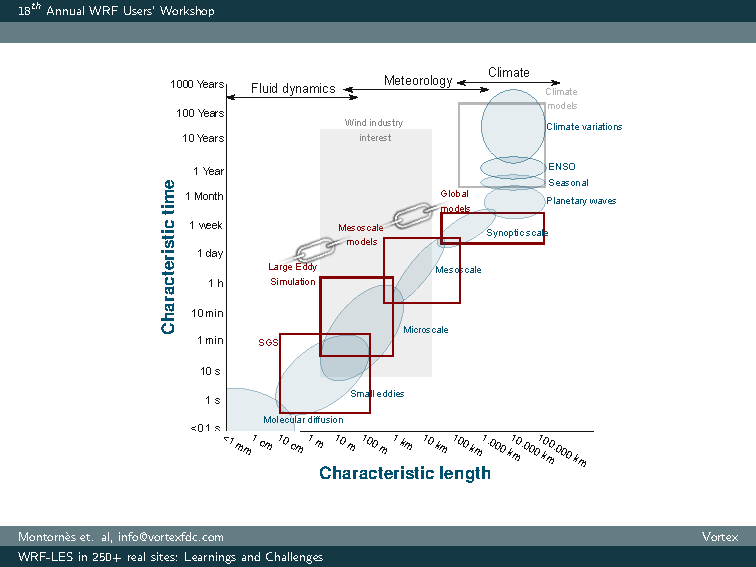
\includegraphics[width=0.7\linewidth,trim={2.6cm 1.4cm 1.5cm 0.8cm},clip]{fig/02/escalas}
		\vspace{-2mm}
		\caption{Unificación de escalas en dinámica atmosférica. Fuente: Montornes et al. (2017).}
	\end{figure}
\end{frame}

\begin{frame}{Motivación}{¿Cómo Predecirlo?}
	\begin{enumerate}[a.]
		\item Extrapolación Estadística / Simulación Numérica.
		\item Modelos Meteorológicos / CFD.
		\item Correcta representación de la CLP (PBL).
		\item Turbulencia y Terreno Complejo.
	\end{enumerate}
\end{frame}

\begin{frame}{Motivación}{¿Cómo Predecirlo?}
\begin{figure}[h]
	\centering
	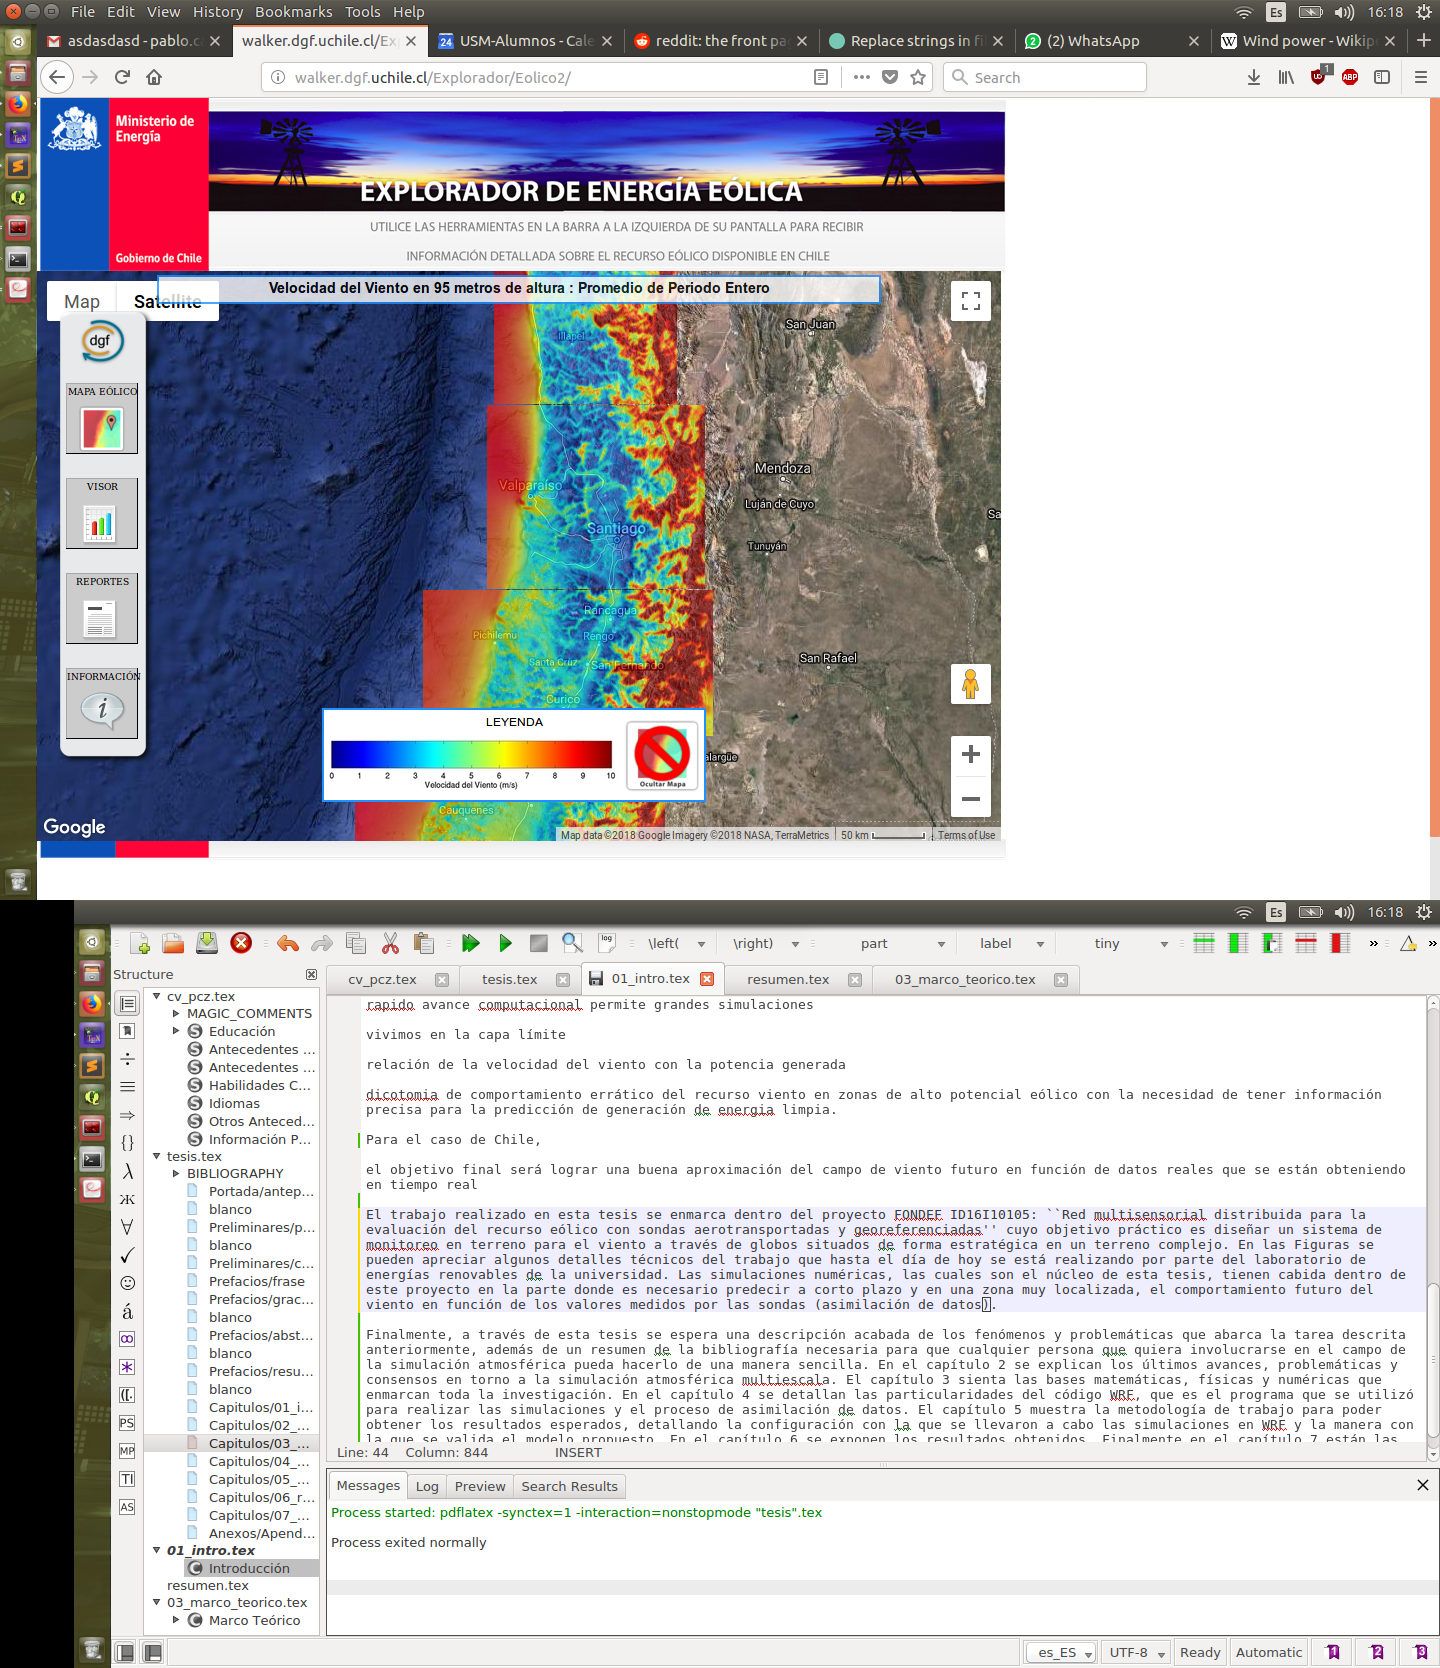
\includegraphics[width=0.8\linewidth,trim={1.4cm 28cm 15cm 3.4cm},clip]{fig/01/explo}
	\vspace{-4mm}
	\caption{Interfaz online del explorador eólico de la Universidad de Chile.}
	\label{fig:01_explorador}
\end{figure}
\end{frame}

\begin{frame}{Motivación}{¿Cómo Predecirlo?}
	\begin{figure}[h]
		\begin{minipage}{0.5\linewidth}
		\centering
		\includegraphics[width=1.0\linewidth,page=5,trim={5cm 9cm 2.3cm 3cm},clip]{fig/01/descrp}
		\end{minipage}%
		\begin{minipage}{0.5\linewidth}
			\centering
			\includegraphics[width=0.9\linewidth,page=5,trim={3cm 2.5cm 5cm 18.5cm},clip]{fig/01/descrp}
		\end{minipage}%
		\caption{Esquema de la sonda FONDEF ID16I10105.}
		\label{fig:01_sonda}
	\end{figure}
\end{frame}

\begin{frame}{Motivación}{¿Cómo Predecirlo?}
	\begin{figure}
		\begin{minipage}{0.5\linewidth}
			\centering
			(a)
		\end{minipage}%
		\begin{minipage}{0.5\linewidth}
			\centering
			(b)
		\end{minipage}%
		
		\begin{minipage}{0.5\linewidth}
			\centering
			\includegraphics[width=0.9\linewidth,page=3,trim={6cm 12.2cm 6cm 9.5cm},clip]{fig/01/descrp}
		\end{minipage}%
		\begin{minipage}{0.5\linewidth}
			\centering
			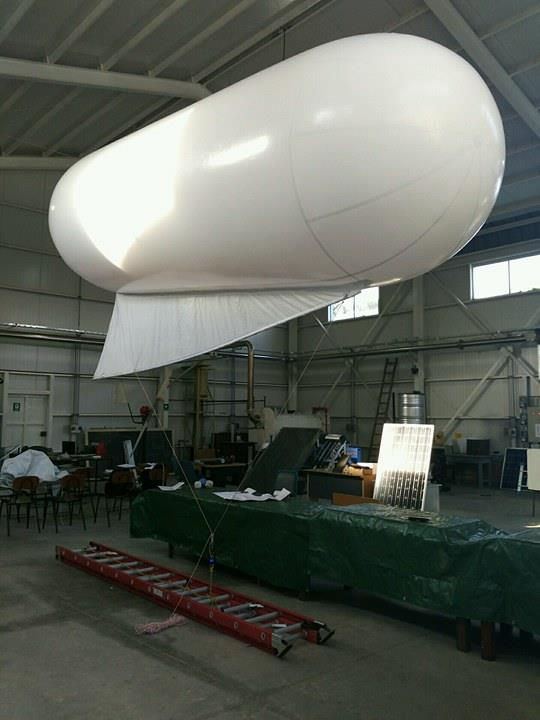
\includegraphics[width=0.7\linewidth,trim={0cm 0cm 0cm 0cm},clip]{fig/01/prototipo}
		\end{minipage}%
		\caption{Detalle del proyecto FONDEF ID16I10105. (a) Célula del sistema experimental de medición. (b) Prototipo en el laboratorio.}
		\label{fig:01_detalle_fondef}
	\end{figure}
\end{frame}

\section{2. Hipótesis y Objetivos}
\begin{frame}{Hipótesis y Objetivos}
	\begin{block}{Hipótesis}\justifying
		Se pueden mejorar las predicciones numéricas de viento a corto plazo sobre terreno complejo a través de simulaciones multiescala de alta resolución, LES y asimilación de datos 4D en la CLP.
	\end{block}
	\begin{block}{Objetivo Principal}\justifying
		Implementar una metodología que incorpore escalamiento dinámico de dominios, nuevas bases de datos de alta resolución, LES y asimilación de datos 4D multipunto para mejorar los resultados de modelos numéricos de viento sobre terreno complejo.
	\end{block}
\end{frame}

\section{3. Estado del Arte}
\begin{frame}{Estado del Arte}
	\begin{enumerate}[a.]
		\item Problemáticas del escalamiento dinámico.
		\item Antecedentes de turbulencia atmosférica y terreno complejo.
		\item Desafios de la alta resolución en terreno complejo.
		\item Contexto de la asimilación de datos.
	\end{enumerate}
\end{frame}

\begin{frame}{Estado del Arte}{Problemáticas del escalamiento dinámico}
	\begin{figure}
		\centering
		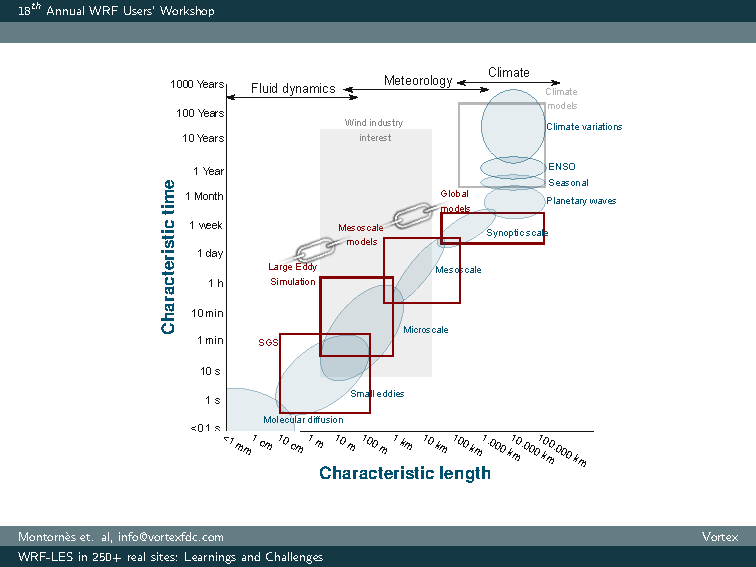
\includegraphics[width=0.7\linewidth,trim={2.6cm 1.4cm 1.5cm 0.8cm},clip]{fig/02/escalas}
		\vspace{-2mm}
		\caption{Unificación de escalas en dinámica atmosférica. Fuente: Montornes et al. (2017).}
	\end{figure}
\end{frame}

\begin{frame}{Estado del Arte}{Problemáticas del escalamiento dinámico}
	\begin{figure}
		\centering
		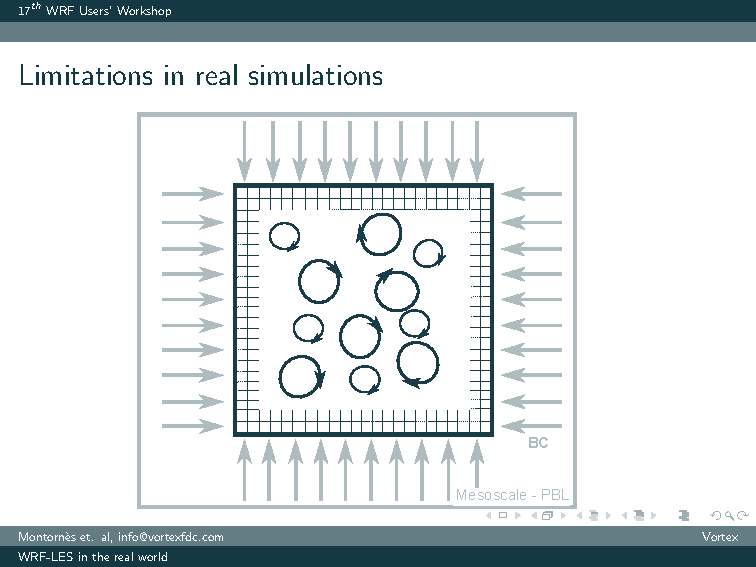
\includegraphics[width=0.6\linewidth,trim={2.67cm 1.35cm 3.1cm 2.25cm},clip]{fig/02/grid}
		\caption{Idealización de los distintos tamaños de vórtices dentro de un dominio en la zona gris de la turbulencia. Fuente: Montornes et al. (2017).}
		\label{fig:02_grid_vortex}
	\end{figure}
\end{frame}

\begin{frame}{Estado del Arte}{Problemáticas del escalamiento dinámico}
	\begin{figure}
		\centering
		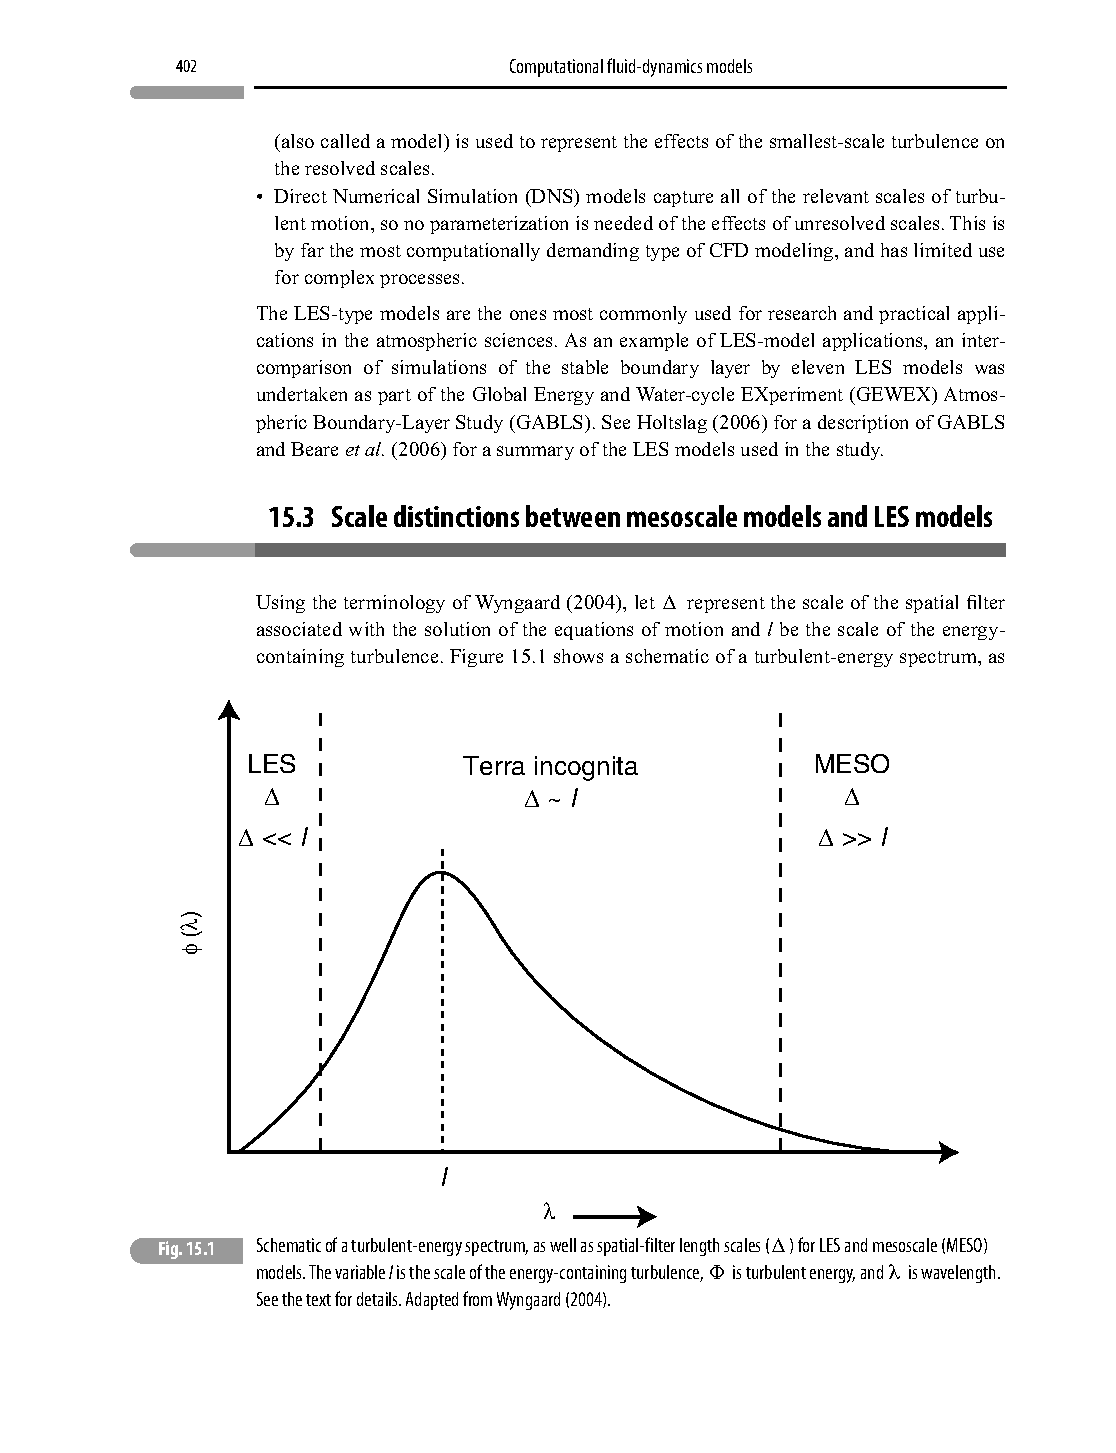
\includegraphics[width=0.9\linewidth,trim={2cm 3.0cm 1.5cm 11.5cm},clip]{fig/02/terra_inc}
		\caption{Espectro de energía cinética turbulenta multiescala. Fuente: Warner (2010).}
		\label{fig:02_terra_inc}
	\end{figure}
\end{frame}

\begin{frame}{Estado del Arte}{Turbulencia Atmosférica y Terreno Complejo}
	\begin{itemize}
		\item aaa
		\item bbb
		\item ccc
	\end{itemize}
\end{frame}

\begin{frame}{Estado del Arte}{Alta Resolución y Terreno Complejo}
	\begin{itemize}
		\item Aspectos Computacionales.
		\item Aspectos Numéricos.
		\item Parametrización de CLP.
		\item Inicialización y Datos de Entrada.
	\end{itemize}
\end{frame}

\begin{frame}{Estado del Arte}{Alta Resolución y Terreno Complejo}
	\begin{figure}[h!]
		\centering
		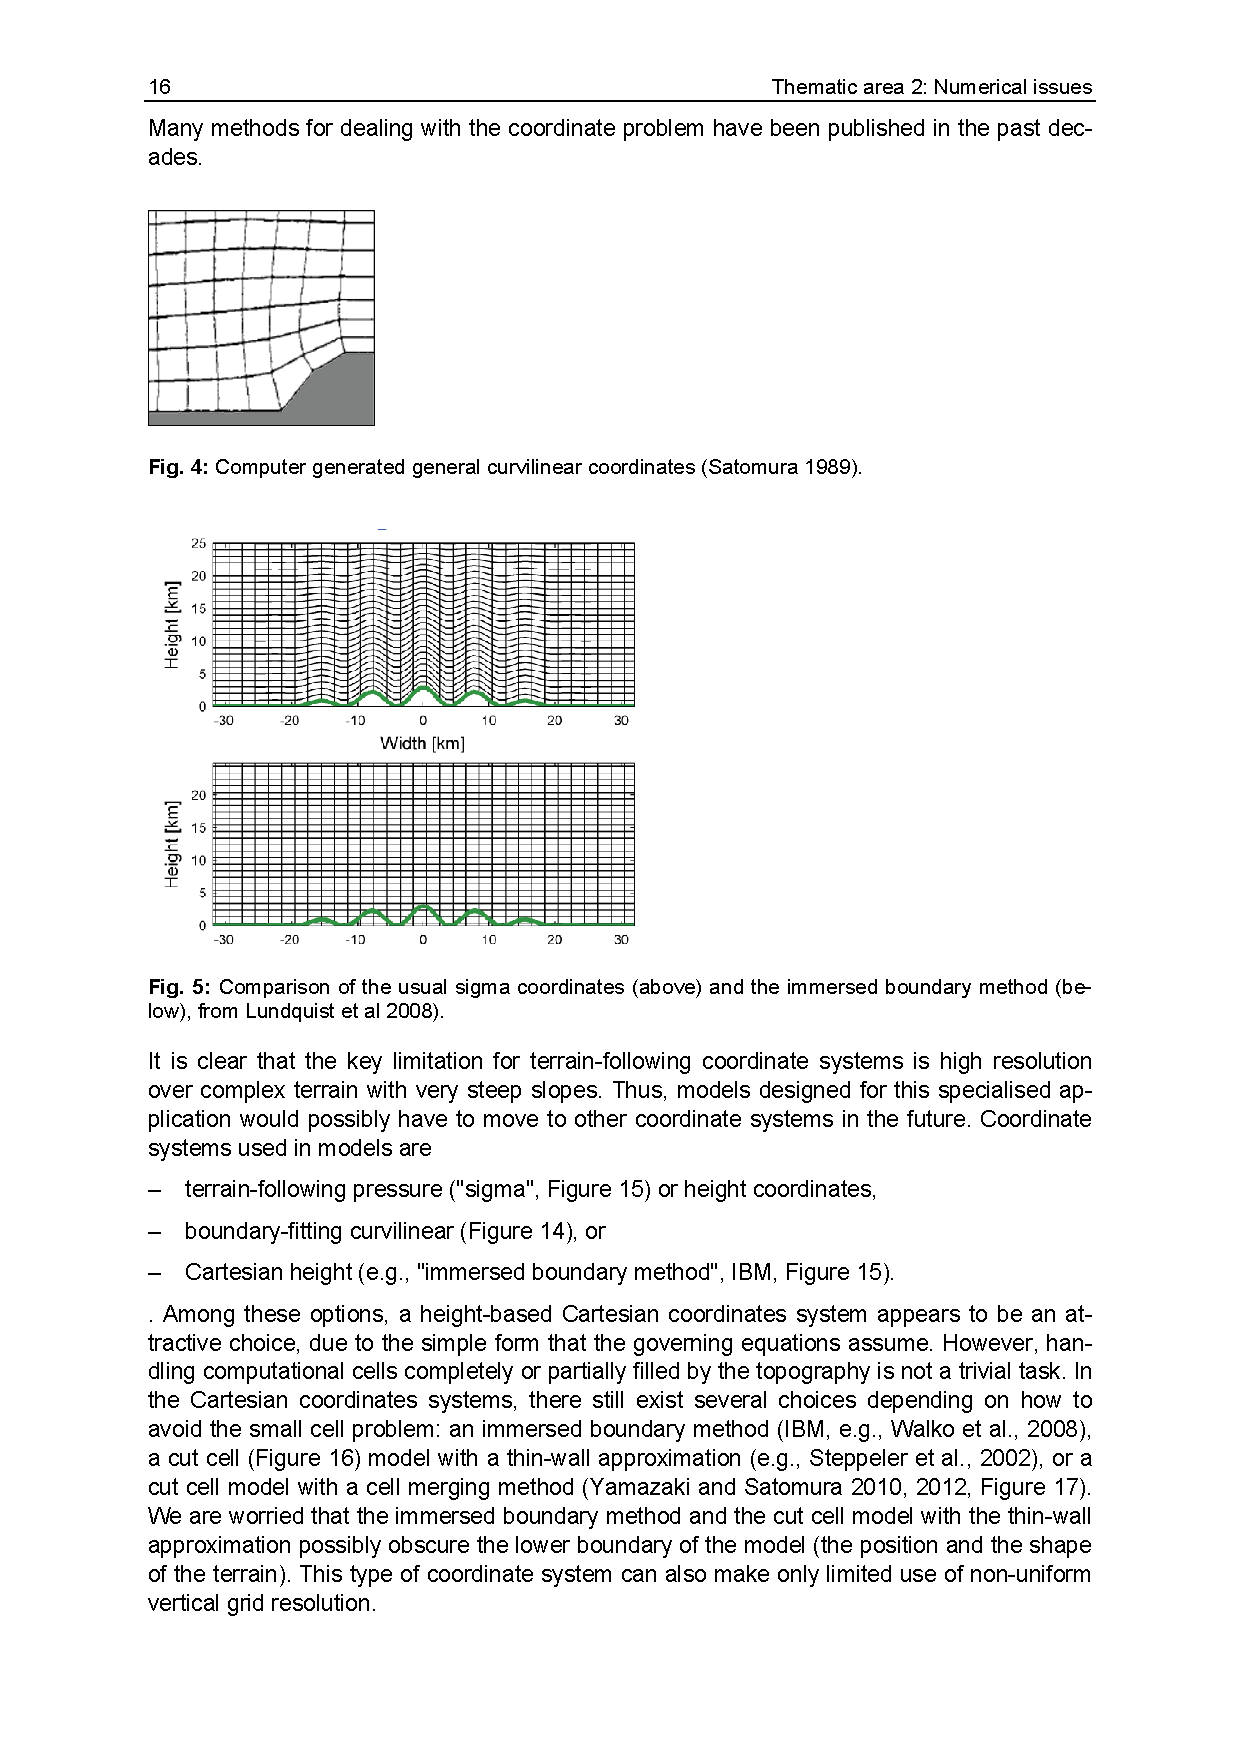
\includegraphics[width=0.75\linewidth,trim={2.6cm 13.5cm 9.2cm 9cm},clip]{fig/02/coordinates}
		\caption{Comparación entre las coordenadas usuales sigma (arriba) y el método de frontera inmersa (abajo). Fuente: Arnold et al. (2010).}
	\end{figure}
\end{frame}

\begin{frame}{Estado del Arte}{Alta Resolución y Terreno Complejo}
	\begin{itemize}
		\item Aspectos Computacionales.
		\item Aspectos Numéricos.
		\item Parametrización de CLP.
		\item Inicialización y Datos de Entrada.
	\end{itemize}
\end{frame}

\begin{frame}{Estado del Arte}{Contexto de la Asimilación de Datos}
	
\end{frame}













\section{4. Marco Teórico}
\begin{frame}{Marco Teórico}
\end{frame}

\section{5. Modelo WRF}
\begin{frame}{Modelo WRF}
\end{frame}

\section{6. Metodología}
\begin{frame}{Metodología}
\end{frame}

\section{7. Resultados}
\begin{frame}{Resultados}
\end{frame}

\section{8. Conclusiones}
\begin{frame}{Conclusiones}
\end{frame}

\begin{frame}{Agradecimientos}
\end{frame}


\begin{frame}
	\vspace{0.3cm}
	\begin{center} 
\includegraphics[height=1.5cm]{utfsm_logo} \end{center}
	\vspace{-0.5cm}
	\titlepage
\end{frame}

\end{document} 